Zu Beginn werden die Apparaturkonstanten $D$ und das Eigenträgheitsmoment $I_\su{D}$
der Drillachse bestimmt.
Dazu wird der Aufbau aus Abbildung \ref{fig:aufbau} verwendet.
\begin{figure}
  \centering
  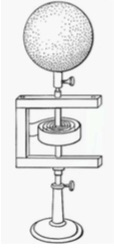
\includegraphics[width=0.2\textwidth]{bilder/aufbau.jpg}
  \caption{Aufbau der Apparatur}
  \label{fig:aufbau}
\end{figure}
Zur Bestimmung von $D$ wird eine nahezu massenlose Stange senkrecht auf die Drillachse gelegt.
Danach wird diese Stange 10 mal um einen Winkel $\varphi$ und dem Abstand $r$
zum Mittelpunkt ausgelenkt und die benötigte Kraft wird mit einem Federmesser
senkrecht zur Stange gemessen. $D$ ergibt sich dann aus Formel \eqref{eqn:D}.
Für $I_\su{D}$ werden zwei Gewichte an diese Stange gehängt und sie wird in Schwingung
versetzt. Auch diese Messung wird 10 mal für verschiedene Abstände $a$ durchgeführt
und die Schwingungsdauer $T$ wird notiert.

Danach wird die Stange nacheinander gegen zwei andere Körper ersetzt, wie z.B.
einem Zylinder oder einer Kugel. Auch diese werden ausgelenkt und die Schwingungsdauer
$T$ wird 5 mal gemessen.
\newpage
Abschließend soll das Trägheitsmoment einer Puppe in zwei verschiedenen Stellungen
bestimmt werden. Dazu wird die Puppe einmal mit angelegten und einmal mit ausgetreckten
Armen auf die Drillachse gespannt, wie in Abbildung \ref{fig:puppe} zu sehen.
Auch bei dieser Messung wird das Trägheitsmoment aus
der Schwingungsdauer bestimmt. Zur Vereinfachung werden die Arme, Beine und der Rumpf
als zylinderförmig und der Kopf als kugelförmig angenommen.
\begin{figure}[!h]
  \centering
  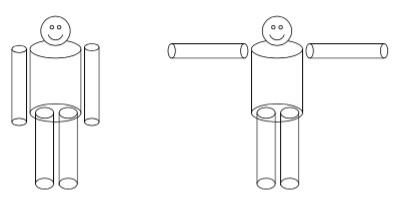
\includegraphics[width=0.8\textwidth]{bilder/puppe.jpg}
  \caption{zwei Stellungen der Puppe}
  \label{fig:puppe}
\end{figure} \\
Wichtig ist es, dass alle verwendeten Körper gewogen und ausgemessen werden.
Zudem müssen die Abstände $a$ zum Schwerpunkt und die Radien $r$ zur Drillachse gemessen
werden und alle Ergebnisse werden gemittelt.
